\section{Message oriented middleware}\label{capitolo6}
RPC e RMI favoriscono un modello di comunicazione di tipo sincrono il quale è un'astrazione più naturale per il programmatore, tuttavia esso supporta solamente interazioni \emph{punto-punto}, inoltre risulta essere molto costoso e richiede un forte accoppiamento tra chiamante e chiamato.\\
Il sistema di comunicazione \emph{asincrono} si incentra sulla nozione di \emph{evento/messaggio}, essa supporta la comunicazione multi-punto e quindi permette un disaccoppiamento tra i componenti. La forma di comunicazione asincrona più diffusa è quella basata sullo scambio dei messaggi, tipicamente gestita direttamente o magari fornita da funzionalità di rete del sistema operativo. Esistono poi dei \emph{Middleware Orientati ai Messaggi} (MOM) che forniscono un'infrastruttura a livello applicativo tra diversi \emph{comunication server}.\\
I MOM forniscono sia comunicazione di tipo sincrono che asincrono, ma l'aspetto fondamentale è che i MOM sono in grado di fornire oltre alla comunicazione di tipo \emph{transiente} nel quale \emph{sender} e \emph{recipients} sono in esecuzione al momento della comunicazione, anche comunicazione di tipo \emph{persistente} nella quale i messaggi vengono immagazzinati dal sistema fino a quando non possono essere recapitati. Esistono due tipologie principali nelle comunicazioni \emph{message oriented}, la prima è la \emph{message queuing} la seconda è il modello \emph{publish-subscribe}; entrambe le tipologie sono orientate ai messaggi, offrono un forte disaccoppiamento tra componenti ed entrambe si basano su di una serie di server per instradare i messaggi e supportare la persistenza.\\
Tuttavia il \emph{message queuing} prevede un tipo di comunicazione punto-punto asincrona e persistente, essa garantisce sempre che il messaggio venga inserito nella coda del destinatario ma non garantisce nulla sul suo comportamento, il sistema risulta perciò disaccoppiato nel tempo e nello spazio e può essere visto come una generalizzazione delle e-mail.
Il sistema risulta essere intrinsecamente peer-to-peer, ogni componente mantiene una coda di input e una di output.
La comunicazione tramite code di messaggi può semplificare anche la comunicazione client server, il client inserisce una richiesta nella coda del server, il server in modo asincrono preleva tale richiesta la processa e restituisce il risultato nella coda del client. Tale meccanismo permette al client di disconnettersi dopo l'invio della richiesta e proseguire nella sua esecuzione, inoltre l'utilizzo delle code permette di semplificare il bilanciamento del carico come si vede in \figurename"\ref{fig:messagequeue}.
\begin{figure}
\centering
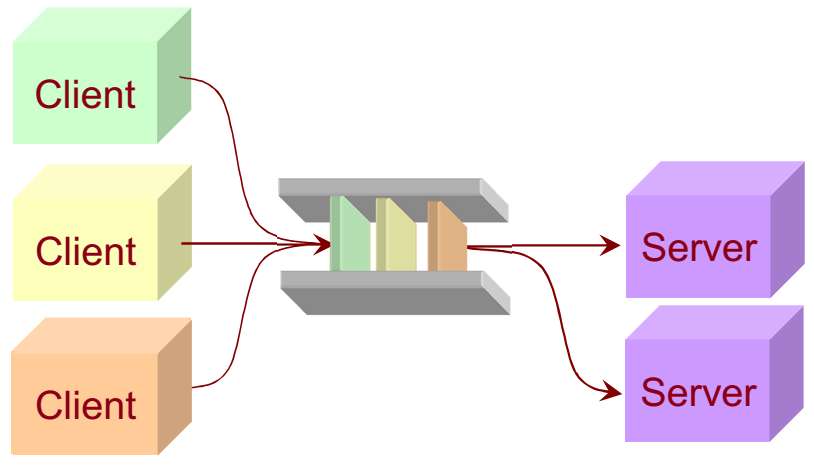
\includegraphics[width=0.7\linewidth]{img/messagequeue}
\caption{Sistema client server basato sulle code di messaggi}
\label{fig:messagequeue}
\end{figure}
Le code sono identificate da nomi simbolici è perciò necessario fornire un servizio di lookup, le code sono gestite da un \emph{queue managers} che può essere locale o remoto.\\
Nella comunicazione \emph{publish-subscribe} i componenti dell'applicazione pubblicano in modo asincrono delle \emph{notifiche}, queste notifiche solitamente sono generate in reazione al verificarsi di un \emph{evento}. I componenti possono dichiarare il loro interesse rispetto a particolari eventi utilizzando un meccanismo di \emph{sottoscrizione}; tali sottoscrizioni sono raccolte da un \emph{event dispatcher} il quale si occupa anche di instradare le notifiche ai diversi sottoscrittori. In base all'espressività del linguaggio di sottoscrizione è possibile distinguere due meccanismi:
\begin{description}
	\item[\emph{Subject-based:}] in questo caso ci si può sottoscrivere ad un insieme ristretto di eventi i cui argomenti sono determinati a priori.
	\item[\emph{Content-based:}] la sottoscrizione contiene un espressione che permette all'event dispatcher di filtrare i messaggi in base al loro contenuto.
\end{description}
\subsection{JMS}
La \emph{Java Message Service} è un API che permette la creazione l'invio, la ricezione  e la lettura dei messaggi all'interno di un sistema enterprise. JMS fornisce tre concetti principali:
\begin{itemize}
	\item \emph{JMS provider:} è l'entità che implementa l'API per la produzione di messaggi
	\item \emph{JMS Client:} è l'applicativo che sfrutta il servizio fornito dal JMS provider.
	\item \emph{JMS domains:} fornisce l'ambiente point-tp-point o publish-subscribe.
\end{itemize}
In JMS esistono dei domini per ogni tipo di comunicazione sia quello point-to-point nel quale ogni messaggio è indirizzato ad una coda specifica e i client estraggono i messaggi da code prestabilite per mantenere i loro messaggi. Il domino di comunicazione publish-subscribe invece è centrato su una gerarchia di topic, JMS, infine mette a disposizione una serie di interfacce indipendenti dal dominio che permettono la comunicazione in entrambi i domini, queste interfacce vengono chiamate \emph{common interface}.\\
Per una trattazione completa si rimandano alle slide dell'insegnante \cite{cugola:jms} un altro tutorial è quello messo a disposizione da Oracle \cite{sun:jms}, infine un implementazione Open Source di jms è JORAM \cite{joram:jms}.
